\documentclass[a4paper]{article}
\usepackage[utf8]{inputenc}
\usepackage[T1]{fontenc,url}
\usepackage{multicol}
\usepackage{multirow}
\usepackage{parskip}
\usepackage{lmodern}
\usepackage{microtype}
\usepackage{verbatim}
\usepackage{amsmath, amssymb}
\usepackage{tikz}
\usepackage{physics}
\usepackage{mathtools}
\usepackage{algorithm}
\usepackage{algpseudocode}
\usepackage{listings}
\usepackage{enumerate}
\usepackage{graphicx}
\usepackage{float}
\usepackage{hyperref}
\usepackage{tabularx}
\usepackage{siunitx}
\usepackage{fancyvrb}
\usepackage[makeroom]{cancel}
\usepackage[margin=2.0cm]{geometry}
\usepackage{pdfpages}
\renewcommand{\baselinestretch}{1}
\renewcommand{\exp}{e^}
\renewcommand{\b}{\boldsymbol}
\newcommand{\h}{\hat}
\newcommand{\m}{\mathbb}
\newcommand{\half}{\frac{1}{2}}
\renewcommand{\exp}{e^}
\renewcommand{\bar}{\overline}
\setlength\parindent{0pt}


\begin{document}
\title{AST5220 -- Milestone I}
\author{
    \begin{tabular}{r l}
        Jonas Gahr Sturtzel Lunde & (\texttt{jonassl})
    \end{tabular}}
% \date{}    % if commented out, the date is set to the current date

\maketitle
\vspace{2cm}

\section{Theory}
\subsection{Components of the universe}
We consider a flat, expanding universe, goverened by the $\Lambda \text{CDM}$ model. Our universe contains some densities of baryonic matter ($\rho_b$), cold dark matter ($\rho_{CDM}$), radiation ($\rho_r$), and dark energy ($\rho_\Lambda$). Let $\Omega_i = \dfrac{\rho_i}{\rho_c}$ be the \textit{relative densities} of each component. Here, $\rho_c$ is the \textit{critical density}, being the total density which would make the universe entirely flat. Since our universe is indeed flat, is follows that
\begin{equation*}
    \sum_i \rho_i = \rho_c \quad \Rightarrow \quad \sum_i \Omega_i = 1
\end{equation*}
We also define $\rho_{i,o}$ and $\Omega_{i,o}$ to represents the critical and relative densities today.

It can be shown that the density components evolve with time as $\rho_i(a) = \rho_{i,0}a^{-3(1+w_i)}$ where $w_i$ is some constant for each component. For our four compoenents, we have that
\begin{align*}
    \rho_b &= \rho_{b,0} a^{-3} \\
    \rho_\text{CDM} &= \rho_{\text{CDM},0} a^{-3} \\
    \rho_r &= \rho_{r,0} a^{-4} \\
    \rho_\Lambda &= \rho_{\Lambda,0}
\end{align*}
where $a$ is the \textit{scale factor} of the universe, describing its relative size to today, which is defined to be $a_0 = 1$.

We wish to avoid the densities where possible, and work directly with the relative densities and the scale factor. The relative densities can be rewritten to exclude $\rho_i$ the following way.
\begin{align*}
    \Omega_{i} = \frac{\rho_i}{\rho_c} = \frac{\rho_{i,0}a^{-3(1+w_i)}}{\rho_c} = \frac{\rho_{c,0}\Omega_{i,0}a^{-3(1+w_i)}}{\rho_c}
\end{align*}

Knowing that $\rho_c = \frac{3H^2}{8\pi G}$, which gives $\rho_{c,0} = \frac{3H_0^2}{8\pi G}$ we get that
\begin{align*}
    \Omega_{i} = \qty(\frac{H_0}{H})^2\Omega_{i,0}a^{-3(1+w_i)}
\end{align*}


\subsection{The Friedmann equation}
The evolution of the scale factor is goverened by the (first) Friedmann equation, which for the universe described above reads
\begin{equation}
    H(a) = \frac{\dot{a}}{a} = H_0\sqrt{\Omega_{b,0} a^{-3} + \Omega_\text{{CDM},0}a^{-3} + \Omega_{r,0}a^{-4} + \Omega_{\Lambda,0}}
\end{equation}

Since the universe takes on scales of many different orders of magnitude, the linear scale factor $a$ is not always well suited for analysis of large time spans. We introduce time(and scale) quantity
\begin{equation}
    x = \log{a} \quad \Rightarrow \quad a = \exp{x}
\end{equation}

The Friedmann equation now reads
\begin{equation}
    H(x) = H_0\sqrt{\Omega_{b,0} e^{-3x} + \Omega_\text{{CDM},0}e^{-3x} + \Omega_{r,0}e^{-4x} + \Omega_{\Lambda,0}}
\end{equation}

We also introduce the scaled Hubble parameter $\mathcal{H} = aH = \dot{a}$.


\subsection{Conformal Time}
As well as $a$, $x$, and $t$ for measuring time in the universe, we will introduce the conformal time $\eta$. $\eta$ has units of length, and represents the size of the event horizon at any given time. In other words, $\eta$ is the distance traversed by undisturbed light since the Big Bang.

[Insert definition of Conformal time]



\newpage
\section{Results}
\begin{figure}[H]
    \centering
    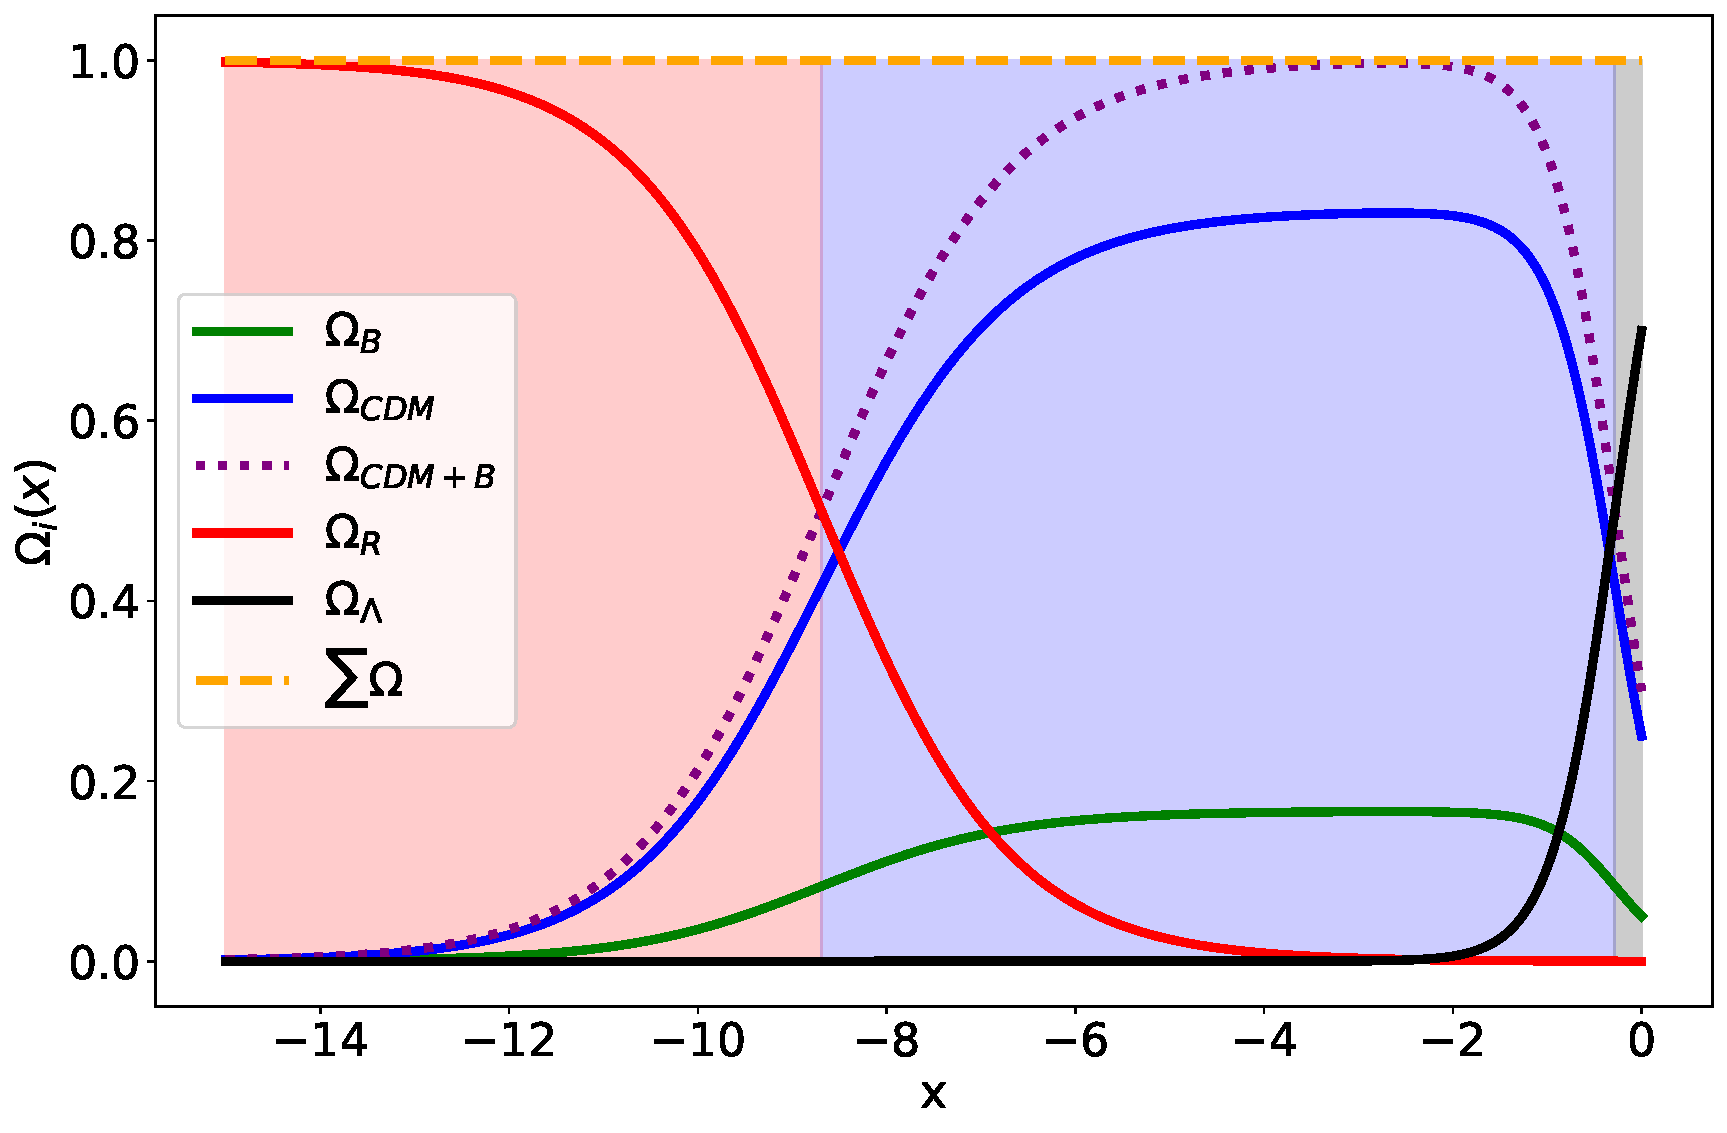
\includegraphics[scale=0.4]{../figs/Omegas.pdf}
    \caption{}
    \label{fig:Omegas}
\end{figure}


\begin{figure}[H]
    \centering
    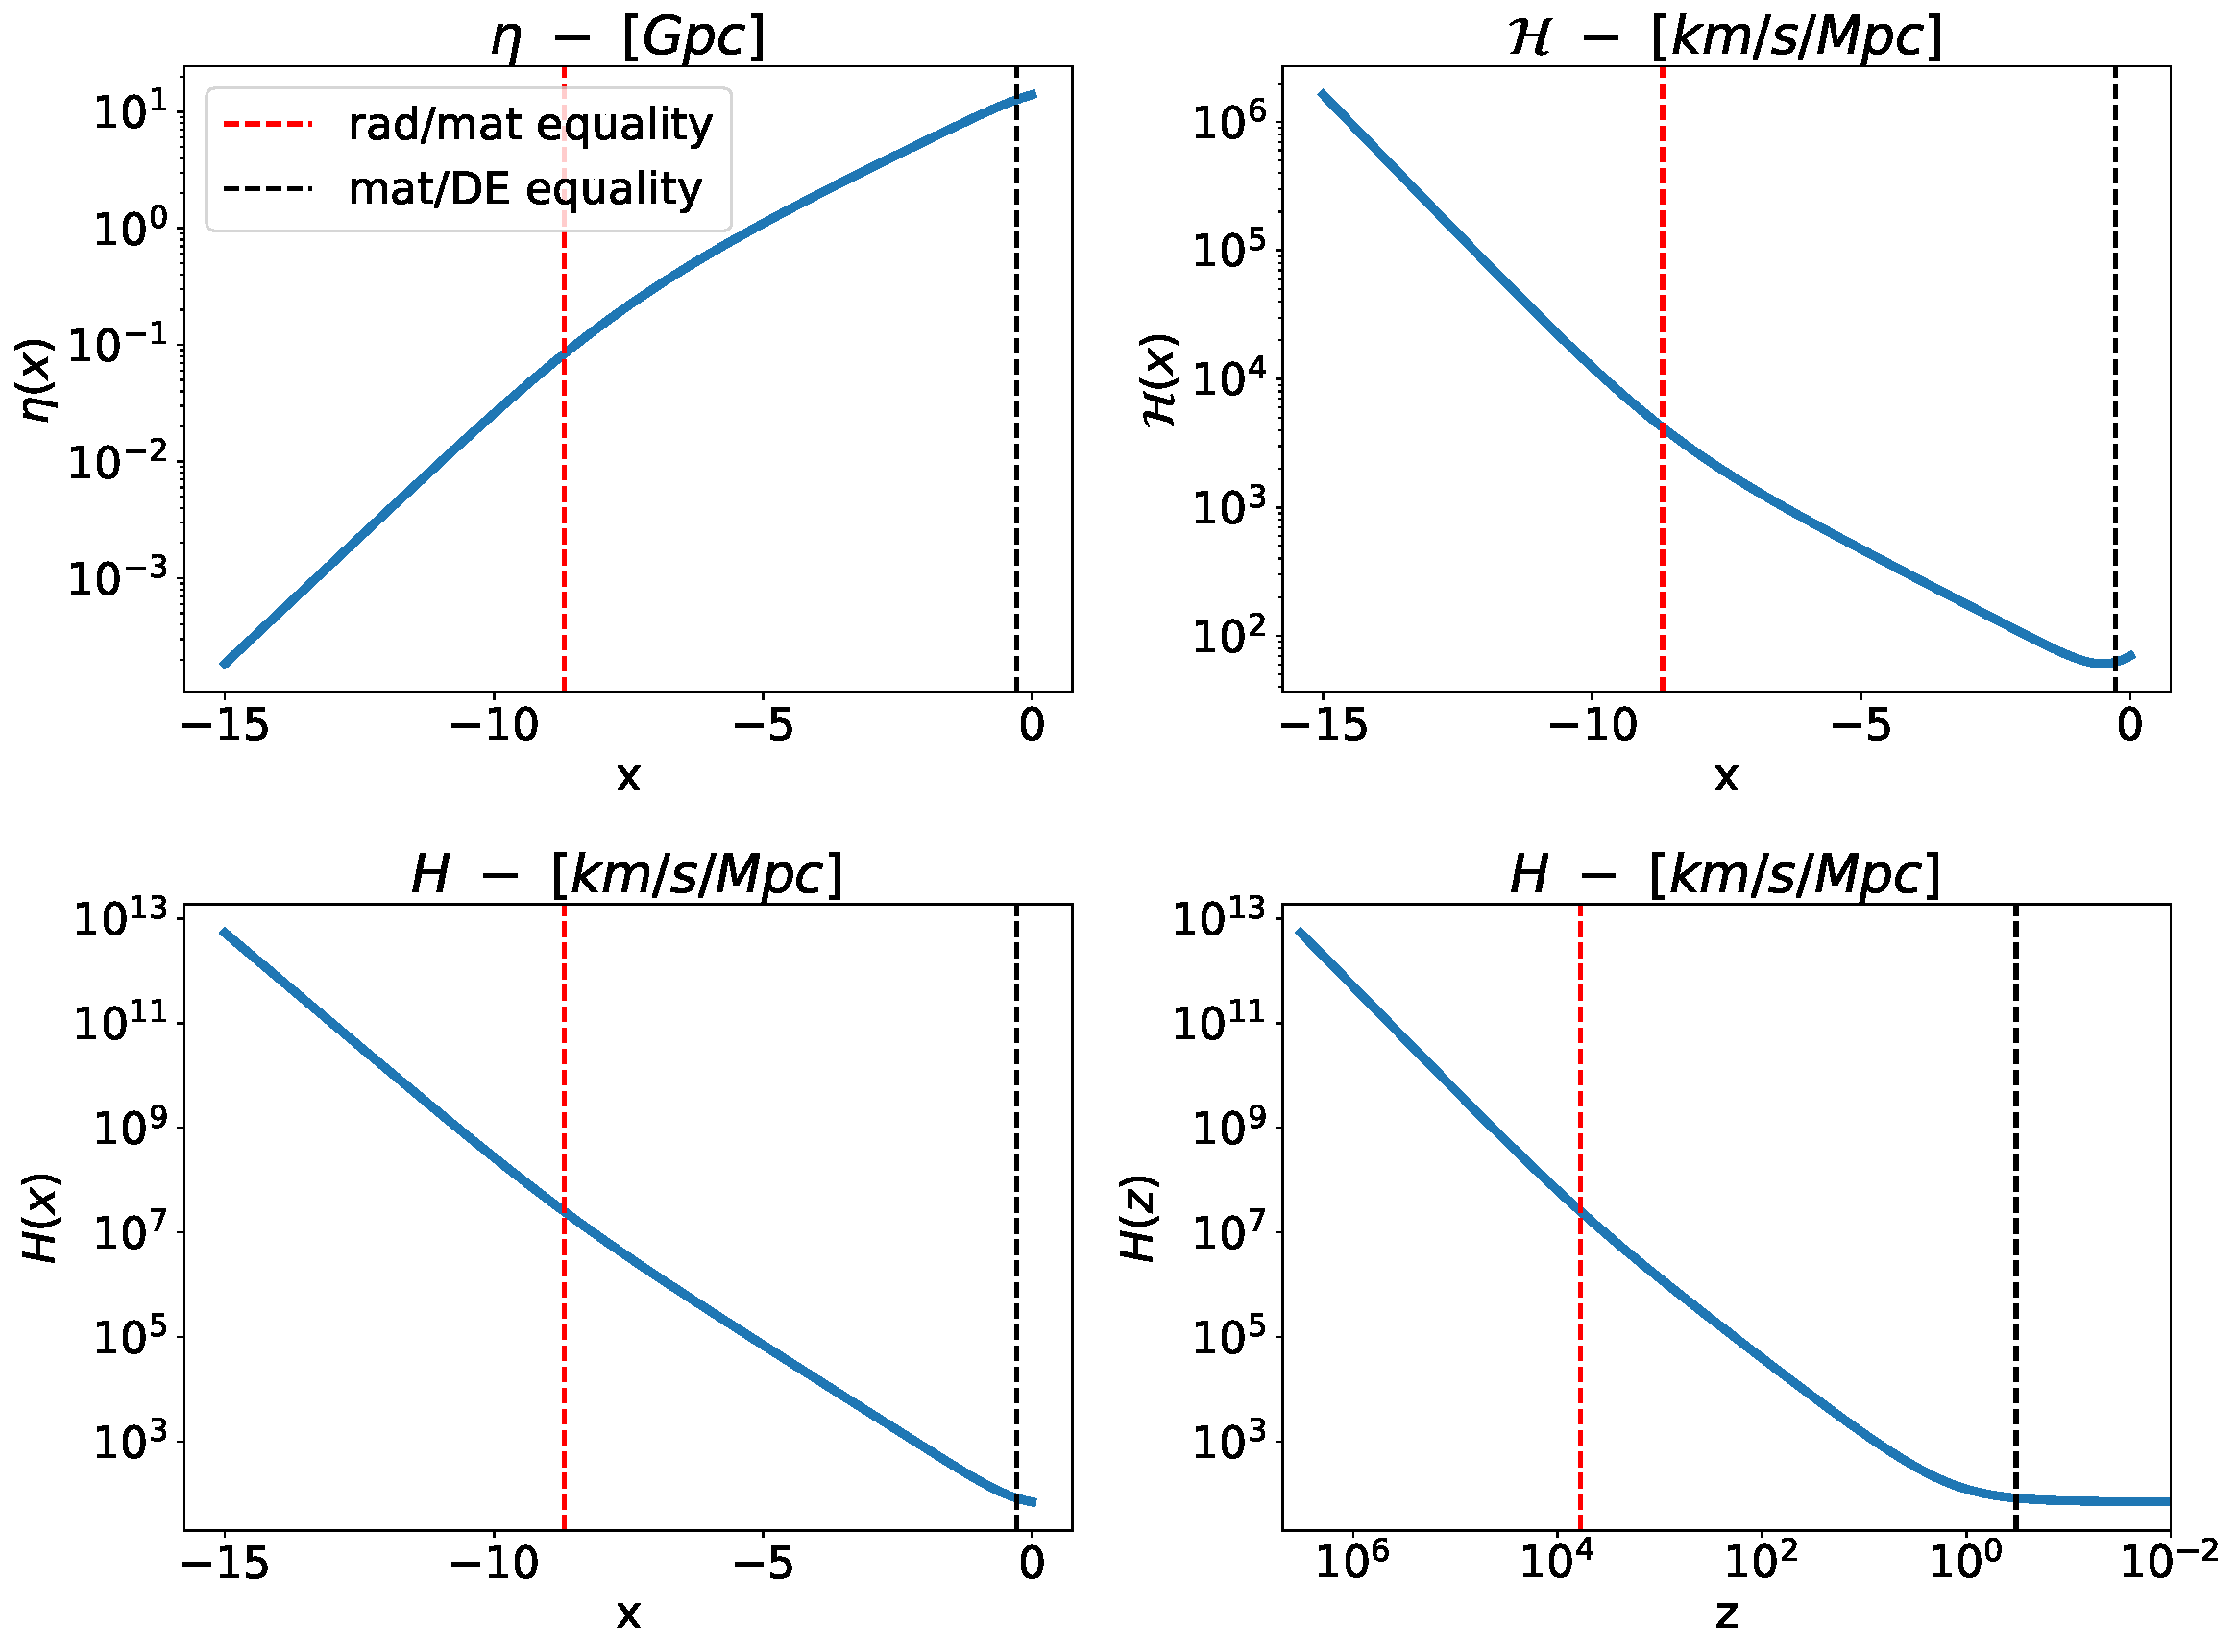
\includegraphics[scale=0.4]{../figs/Eta.pdf}
    \caption{}
    \label{fig:Eta}
\end{figure}




\end{document}